%
%  conceitos
%
%  Created by Thadeu Carmo on 2010-09-04.
%  Copyright (c) 2010 __MyCompanyName__. All rights reserved.
%
\documentclass[]{article}

% Use utf-8 encoding for foreign characters
\usepackage[utf8]{inputenc}

% Setup for fullpage use
\usepackage{fullpage}

% Uncomment some of the following if you use the features
%
% Running Headers and footers
%\usepackage{fancyhdr}

% Multipart figures
%\usepackage{subfigure}

% More symbols
%\usepackage{amsmath}
%\usepackage{amssymb}
%\usepackage{latexsym}

% Surround parts of graphics with box
\usepackage{boxedminipage}

% Package for including code in the document
\usepackage{listings}

% If you want to generate a toc for each chapter (use with book)
\usepackage{minitoc}

% This is now the recommended way for checking for PDFLaTeX:
\usepackage{ifpdf}

\usepackage{indentfirst}
%\newif\ifpdf
%\ifx\pdfoutput\undefined
%\pdffalse % we are not running PDFLaTeX
%\else
%\pdfoutput=1 % we are running PDFLaTeX
%\pdftrue
%\fi
\newtheorem{prop}{Proposição}[section]

\ifpdf
\usepackage[pdftex]{graphicx}
\else
\usepackage{graphicx}
\fi
\title{Conceitos Básicos e Anotações Importantes}
\author{Thadeu de Russo e Carmo}

\date{2010-09-04}

\begin{document}

\ifpdf
\DeclareGraphicsExtensions{.pdf, .jpg, .tif}
\else
\DeclareGraphicsExtensions{.eps, .jpg}
\fi

\maketitle


\begin{abstract}
	Este documento foi escrito e é constantemente atualizado para me ajudar a não esquecer os conceitos básicos, bem como
	colocar resumos importantes sobre as leituras feitas.
\end{abstract}

\section{Lei de Gordon Moore}
	\par Tudo começa com a lei de Gordon E. Moore, que descreve uma tendência de longo prazo para a quantidade de transistores
	que podem ser colocados em uma chip. Esta tendência mostra um crescimento exponencial a cada dois anos, e vem desde
	1965 se confirmando, sem espectativa de mudanças até 2015 \cite{Moore1965} \cite{MooreLaw}. 
	
	\subsection{Consequências}
	\par O aumento exponencial do número de transistores nos processadores não implica em um aumento também exponencial
	no poder
	de processamento (no texto da Wikipedia, tem um caso onde 45\% de aumento nos transistores do processador mostraram apenas
	um aumento entre 10\% a 20\% no poder de processamento.\cite{DothanInvestigated}). A velocidade de um sistema não é
	afetada somente pela velocidade do processador, mas por outros fatores como, por exemplo, largura de banda interna e
	velocidade de armazenamento. Ainda é citado que a velocidade de acesso a disco não acompanhou a evolução da velocidade
	dos processadores, sendo apontado como um gargalo.
	
	\subsection{The Free Lunch}
		\par De acordo com o texto, por anos fabricantes de processadores entregaram processadores com \textit{clocks} mais
		rápidos e paralelismo a nível de instruções, de modo que códigos \textit{single-thread} pudessem ser executados mais
		rápido sem modificações \cite{Shutter2005} (O texto escrito é um enorme resumo da primeira parte do artigo). 

	\subsection{The Free Lunch is Over!}
		\par Existe uma barreira física que coloca uma barreira no aumento da velocidade de \textit{clock} dos processadores.
		No texto da Wikipedia, o autor menciona que para gerenciar a dissipação de energia. Neste artigo ele não menciona os
		detalhes da limitação física, mas apresenta um gráfico mostrado na figura ~\ref{fig:cpu_chart}, que deixa bem claro
		o que acontece.
		
		\vspace{1ex}
		\begin{figure}[hbtp]
		\centering
		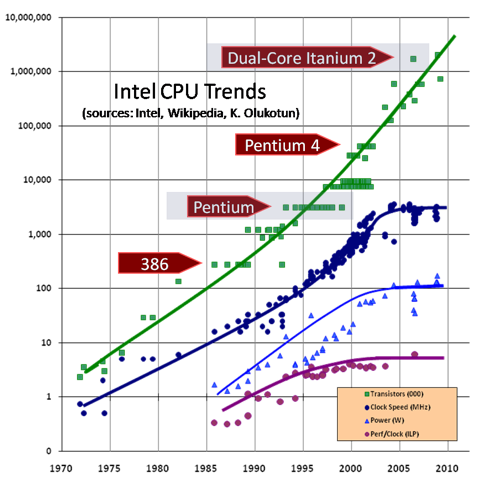
\includegraphics{images/cpu-chart.png}
		\caption{Processador Intel - velocidade de clock por transistores}
		\label{fig:cpu_chart}
		\end{figure}
		
		\par O que muda do ponto de vista de \textit{software}? Simples: programas \textit{single-thread} não 
		conseguirão pegar carona (= ficar mais rápidos) nos processadores com múltiplos núcleos como até então
		haviam feito durante anos nos processadores com um único núcleo. Isso implica no fato que para que os
		programas sejam mais rápidos (= tirem vantagem dos múltiplos núcleos), devem ser escritos com múltiplas
		\textit{threads} ou processos. No texto ele enumera os seguintes pontos (o texto é de 2005):
		\begin{enumerate}
			\item Claramente as aplicações deverão ser concorrentes se elas quiserem explorar
			totalmente os ganhos da nova geração de processadores\footnote{			
			 The clear primary consequence we’ve already covered is that applications will increasingly need to be
			 concurrent if they want to fully exploit CPU throughput gains that have now started becoming available and will
			 continue to materialize over the next several years. For example, Intel is talking about someday producing
			 100-core chips; a single-threaded application can exploit at most 1/100 of such a chip’s potential throughput.};

			\item Menos óbvio, porém importante, é o fato de que aplicações serão, provavelmente limitadas pelas CPUs
			\footnote{
			Perhaps a less obvious consequence is that applications are likely to become increasingly CPU-bound. Of
			 course, not every application operation will be CPU-bound, and even those that will be affected won’t become
			 CPU-bound overnight if they aren’t already, but we seem to have reached the end of the “applications are
			 increasingly I/O-bound or network-bound or database-bound” trend, because performance in those areas is still
			 improving rapidly (gigabit WiFi, anyone?) while traditional CPU performance-enhancing techniques have maxed
			 out.};
			
			\item Otimização de eficiência e desempenho serão mais importantes
			\footnote{
				Efficiency and performance optimization will get more, not less, important. Those languages that already
			 lend themselves to heavy optimization will find new life; those that don’t will need to find ways to compete and
			 become more efficient and optimizable. Expect long-term increased demand for performance-oriented languages and
			 systems.};
			
			\item Linguagens de programação e sistemas serão forçados a lidar bem com concorrência
			\footnote{
			Programming languages and systems will increasingly be forced to deal well with concurrency. The Java
			 language has included support for concurrency since its beginning, although mistakes were made that later had to
			 be corrected over several releases in order to do concurrent programming more correctly and efficiently. The C++
			 language has long been used to write heavy-duty multithreaded systems well, but it has no standardized support
			 for concurrency at all.}.
		\end{enumerate}
		
\section{Concorrência em Software}		
	\par Com a necessidade (obrigação?) de se escrever programas concorrentes, um antigo problema volta à tona: estado
	compartilhado (no texto ele chama de \textit{sharing unstructured state}). Quando duas tarefas tentam acessar o mesmo
	objeto, e uma consegue modificar o seu estado, se não coordenarmos as tarefas, teremos uma condição  chamada de
	\textit{data race}, algo que de longe não é bom já que as tarefas podem estar lendo/escrevendo dados inconsistentes
	ou corrompidos. Uma das maneiras de se evitar \textit{race conditions}, é através do uso de \textit{locks}.
	
	
	\subsection{Locks e seus problemas}

	\subsubsection{O funcionamento}
		\par O funcionamento de um \textit{lock} é simples: toda tarefa que deseja executar um conjunto de operações em
		uma parte de memória compartilhada deve, obrigatoriamente, obter o \textit{lock} relacionado àquela parte, 
		executar as operações e liberar o \textit{lock} para que outras tarefas também possam executar suas tarefas.
	
	\subsubsection{Problemas}
		\par Os problemas são listados a seguir:
		\begin{itemize}
			\item \textbf{Não componibilidade}: Não é possível se obter mais de um \textit{lock}, combiná-los e saber
			se o resultado ainda está correto. O desenvolvimento de software moderno é depende fortemente da habilidade
			de se compor bibliotecas formando grandes programas, sendo uma enorme dificuldade não se poder construir
			sobre bibliotecas baseadas em \textit{locks}, sem analisar suas implementações;

			\item \textbf{Deadlocks}: Consequência da não-componibilidade de \textit{locks}. Ocorre quando duas travas
			precisam ser adquiridos em order contrária. Suponha que a tarefa T1 tem o \textit{lock} L1 e que T2 tem L2. 
			T1 precisa adquirir L2 e T2 precisa adquirir L1. A definição usada no texto do Agha é a seguinte: 
			``Deadlock é a condição onde não há processo capaz de se comunicar com outro". No texto do Simon Jones (e na
			qualificação), existe uma lista legal que aponta algumas dificuldades como: Esquecimento de travas,
			obtenção de travas em excesso, obtenção de travas erradas, obtenção de travas na ordem errada, liberação de
			travas perante a falhas, esquecimento de sinalização ou verificação de variáveis de condição;
			
			\item \textbf{LiveLocks}: Caso clássico de \textit{starvation}. O processo não faz progresso algum.
					
		\end{itemize}
	
		\par Existem outros problemas não diretamente relacionados a \textit{locks}, como divergência (= loop infinito).
		O texto do Sutter menciona que linguagens imperativas, que usam estruturas de controle com granularidade fina e
		manipulações de dados de baixo-nível, fazem com que programas nestas linguagens sejam difíceis de se analizar
		e paralelizar automaticamente.\\

		\par Os grandes pontos fortes das linguagens funcionais, no que diz respeito a concorrência são:
		\begin{enumerate}
			\item Manipulam instâncias imutáveis;
			\item Programas side-effect free;
			\item O paralelismo exposto fica a nível de chamadas de \textit{procedures};
			\item Estilo de programação de alto nível (e.g.: map, map-reduce, forall). Operações de alto nível são
			fontes ricas de concorrência;
		\end{enumerate}		
		
	\subsection{STM}
		-- A parte de STM vai esperar um pouco, preciso focar em atores.
	\subsection{Abstrações de alto nível}
		Três exemplos de abstrações de alto nível que o Sutter menciona no texto dele são asynchronous calls, 
		futures e active objects (este tem implementação no Akka).
		\subsubsection{Asynchronous calls}
			Uma chamada assíncrona é uma chamada de função ou método não bloqueante. O \textit{caller} continua
			executando e, conceitualmente, uma mensagem é enviada para uma tarefa ou \textit{fork}, para executar
			a operação de maneira independente.
		\subsubsection{Futures}
			Um \textit{future} é um mecanismo  para retorno de resultados de uma chamada assíncrona; ele age como um
			placeholder para o valor que ainda não foi materializado.
		\subsubsection{Active Objects}
			Conceitualmente um \textit{active object} executa em sua própria thread, logo criar $1000$ \textit{active objects}
			criariam $1000$ potenciais threads de execução. Um \textit{active object} age como um monitor, de modo que
			apenas um método do objeto é executado em um dado momento, porém não é necessário o \textit{locking} tradicional.
			Chamadas de métodos externas são enfileiradas e processadas pelo objeto.
		
	\subsection{Modelo de Atores}

		\par Segundo o texto do Agha, um ator é um agente computacional que mapeia cada comunicação recebida em uma
		3-tupla consistindo de:
		\begin{enumerate}
			\item Um conjunto finito de comunicações enviado para outros atores;
			\item Um novo comportamento, que será usado na resposta da comunicação seguinte;
			\item Um conjunto finito de novos atores criados.
		\end{enumerate}

		\par Como observações importantes são destacados que o comportamento de um ator pode ser sensitivo ao histórico,
		que não há sequencialidade presumida nas ações que o ator executa (cada uma das suas ações é uma função do
		comportamento do ator e das comunicações recebidas) e que a criação de um ator é parte do modelo. Ele comenta
		também (depois de uma considerável argumentação) da necessidade de a comunicação ser assíncrona e da necessidade
		de buffers para tal. Fala sobre o não-determinismo na entrega de mensagens, dizendo que não é possível se prever
		exatamente quando uma comunicação enviada por um agente vai ser recebida por outro, por vários fatores (basicamente
		dinamismo e reconfigurações). Sobre a garantia de entrega, ele se baseia na física para dizer que não faz sentido
		uma determinada comunicação não ser entregue e joga a responsabilidade para quem for construir o sistema, porém não
		diz que todas as mensagens deve significantemente processadas (aqui tem a diferença dos Erlang Actors e Scala Actors
		para os Akka Actors). Ele argumenta sobre a justiça (\textit{fairness}), e diz que garantia de entrega não
		é o bastante, ja que as mensagens não devem ser simplesmente entregues, pois seu processamento pode facilmente
		gerar um caso de loop infinito. E.g.: Ator recebe uma mensagem \emph{short} e no seu processamento, se auto-envia
		uma mensagem \emph{short}. Ator recebe uma mensagem \emph{short} e uma \emph{long} concorrentemente. Garantia
		de entrega nao garante que a mensagem \emph{long} possa vir a ser processada.\\
		
		\par Computação em um sistema de atores acontece em resposta a comunicações enviadas para o sistema. Comunicações
		são contidas em tarefas (ele usa tasks). Uma tarefa é representada como uma 3-tupla:
		\begin{enumerate}
			\item Uma Tag para distinguir a task das outras tasks do sistema (um identificador único);
			\item Um Target que é o endereço da caixa de correio no qual a comunicação será entregue;
			\item A comunicação que possui a informação que o ator irá processar.			
		\end{enumerate}		

		\par É importante destacar que o Target deve ser um endereço valido e conhecido antes do envio, que um ator só
		pode processar tasks cujos targets correspondam ao seu endereço, para qualquer ator, a ordem de chegada das
		mensagens deve ser linear -- deve haver uma maneira de tratar o caso onde duas comunicações chegam ao mesmo
		tempo. Um ator pode ser descrito por especificar:
		\begin{enumerate}
			\item O endereço da sua caixa de correio;
			\item Seu comportamento, que é uma função da comunicação aceita.
		\end{enumerate}
		
		\par Quando um ator $X_n$ aceita a $n^{th}$ comunicação em sua caixa de mensagens, ele pode criar tanto outros
		atores ou tasks, e em seguida criará um novo ator $X_{n+1}$ substituto que irá processar a comunicação
		$n^{st+1}$ (que pode já estar na caixa de mensagens ou não). Ainda é possível  que $X_n$ ainda esteja no
		processo de criação mais tasks e outros atores ainda que $X_{n+1}$ esteja fazendo o mesmo (ou seja, eles podem
		estar processando mensagens em paralelo). Em qualquer um dos casos, note que $X_n$ não receberá futuras 
		comunicações e nem criará outro substituto.
		
		\par As vezes o comportamento de um ator substituto pode depender de comunicações com outros atores (no texto,
		ele cita o exemplo de um saque que vai depender uma verificação com uma conta poupança). Ele da detalhes
		de como se implementar isso, porém o que eu entendi é que no meio tempo que não se sabe o comportamento
		substituto, o ator fica \emph{insensível} (insensitive) e apenas armazena (na verda, encaminha para o buffer)
		as mensagens, sem processamento. Outro termo que ele usa é o de Atores Primitivos, que basicamente são atores
		com comportamento estático.

		
		\par Como o modelo de atores se comporta em alguns dos problemas (clássicos e que fazem sentido quando não
		estamos trabalhando com locks) de concorrência, listados a seguir.
		
		\subsubsection{Divergência}
		\par Normalmente chamada de loop infinito. Gostariamos de ter um programa com, potencialmente computações
		infinitas (como um relógio, ou um monitorador), mas que ainda assim pode ser terminado ou reinicialidado de
		maneira graciosa. Tem um outra definição que chama de \textit{endless chatter} (tagarelagem sem fim). O
		exemplo é dado com o código de um relógio, onde caso uma mensagem `go' seja recebida, ele dispara a contar
		incrementando seu valor em $1$. Caso qualquer outra mensagem seja recebida, ele volta a contar a partir de $0$.
		Neste caso, a garantia de entrega do modelo nos da a certeza que o relógio pode ser reiniciado. O caso
		da tagarelagem sem fim, mesmo para atores com comportamento não estático, também é resolvido com a garantia
		de entregua das mensagens.
		
		\subsubsection{Deadlock}
		\par Pela definição do Brookes, em linguagens que usam comunicação síncrona de mensagens, deadlock é definido
		como sendo uma condição onde não há processo capaz de se comunicar com outro. Uma outra definição diz que
		um deadlock é uma situação onde não é possível ocorrer uma evolução do sistema. Caso clássico definido
		por Dijkastra é o problema dos filósofos.

		\par No modelo de atores, este problema é enderaçado de duas maneiras. Primeiro que deadlocks sintáticos 
		(baixo-nível) não são possíveis no modelo, no sentido de ser impossível a comunicação (como na definição do
		Brookes). No caso do exemplo dos filósofos, o chopstick, mesmo em uso deve designar um substituto, e este
		substituto pode `responder' a consulta de um filósofo. Importante: No caso de um filósofo ser programado
		para ficar simplesmente tentando pegar um chopstick, do ponto de vista \emph{semântico} o sistema estaria
		em deadlock. Contudo, o chopstick substituto poderia responder quem está usando o chopstick, e o filósofo
		que deseja pegar o chopstick consultar diretamente quem o está usando (que é por quem se está esperando).
		A condição que causaria um deadlock seria de o filósofo estar esperando por si próprio. O maior problema
		em relação a deadlocks é identificá-los. No texto ele diz que atores podem identificar esta situação, 
		consultando outros atores sobre o estado que estão. Os filósofos, mesmo estando `ocupados' (seja comendo ou 
		procurando por chopsticks), ainda assim por conta da garantia de entrega do modelo, conseguem receber 
		comunicações e o sistema consegue evoluir.
		
		\subsubsection{Exclusão Mútua}
		\par Pode-se dizer que exclusão mútua é uma necessidade que surge quando mais de um processo deseja
		acessar um recurso compartilhado, e na abordagem clássica, é resolvido com um mutex. Um ator representa
		total encapsulamento e só pode ser `acessado' pelo envio de comunicações e podemos, seguramente dizer que
		não é um problema para o modelo de atores.
		
		\subsubsection{Atomicidade}
		\par Atomicidade é possível no modelo de atores com o uso de recepcionistas. Estes que por sua vez
		limitam a interface do sistema com o mundo exterior. Como exemplo, o Agha usa uma conta bancária que
		pode ser acessada por diversos clientes. Neste exemplo o conjunto de transações de um determinado cliente
		deve ser atômico. A solução usa um ator recepcionista chamado \textit{account-receptionist} que, de certo
		modo, encapsula ou esconde o ator que representa a conta do mundo exterior e cuida para que não haja 
		intercalação dos eventos vindos dos diferentes usuários. Um ponto importante é que não existe um nível
		pré-determindado de granularidade para atomicidade no modelo, ficando a cargo do programador definir isso.
		
		\subsubsection{Componibilidade}
		\par No texto o Agha fala sobre o que é dito como sendo componibilidade em CCS. Aparecem termos como
		\emph{portas},\emph{portas complementares} (portas que podem ser ligadas). Quando a conversa vem para
		o nível de atores, ele fica fazendo comparações com CSS e o que da para concluir é que atores são vistos
		como uma comunidade de agentes com \emph{endereço} fixo (a caixa de correio) e podem receber diversas 
		comunicações e a única sequêncialidade definida é consequência de interações causais.
		
		\par Relacionado a componibilidade, volta o assunto de recepcionistas que podem ser usados para encapsular
		atores do mundo exterior. Vale lembrar que um ator só pode receber comunicações de outros atores que 
		conheçam de antemão seu endereço de correio. No texto ele levanta 3 pontos que não são complicados de se
		concluir sobre o uso de recepcionistas para encapsulamento.
		\begin{enumerate}
			\item Atores recepcionistas podem ser conhecidos por outros atores do sistema, e comunicações internas
			não são vistas pelo mundo externo;
			\item Novos recepcionistas podem ser criados como evolução do sistema. Novos recepcionistas são criados,
			basicamente informando os endereços de suas caixas de correio para o mundo externo;
			\item  Recepcionistas não poder ser arbitrariamente restritos. Uma vez que um endereço é conhecido pelo
			mundo exterior, o ator se torna um recepcionista. Uma vez que o endereço deixa de ser conhecido, o ator
			deixa de ser um recepcionista.
		\end{enumerate}
		
		\par Componibilidade no modelo de atores é possível através da troca de mensagens. Sistemas independentes são
		conectados (compostos) por enviar a alguns atores externos de cada módulo uma comunicação para se tornarem
		atores encaminhadores, que simplesmente enviam o endereço de suas caixas de correio para alguns recepcionistas 
		do outro módulo. No texto ele define e prova a seguinte proposição:
		
		\begin{prop}
			Se o comportamento de um ator $x$ nunca muda (a.k.a unserialized), e seu comportamento é encaminhar
			todas as comunicações que ele aceita para um ator $y$, então enviar uma comunicação para $x$ é 
			equivalente a enviar uma comunicação para $y$.
		\end{prop}
		\par Para provar formalmente a proposição, é necessário mostrar que dada uma configuração com um ator 
		encaminhador, podemos construir uma configuração equivalente sem este ator, fazendo uma substituição
		do endereço da caixa de correio dele na lista de conhecimento de todos os atores e tarefas na configuração
		pelo endereço da caixa de correio do ator que ele encaminha as comunicações que ele recebe. Ele menciona
		e se baseia também nos fatores da garantia de entrega e não-determinisno na ordem de chegada das mensagens.
		Ele ainda vai fundo nas \textit{contraints} da composição de duas configurações.
		
		\subsubsection{Problemas}
		\par Os principais problemas levantados em relação ao modelo de atores estão ligados a perda de linearidade
		(chamada de inversão de controle) no código e na dificuldade de se fazer testes unitários por conta da
		característica assíncrona (aqui vale a pena eu olhar os testes unitários do Akka).
	\subsection{MOMs e AMQP}
		\subsubsection{MOMs}
			No livro de web services do Alonso, ele comenta que MOMs são frequentemente apontados como uma tecnologia
			que pode mudar o modo como sistemas  distribuídos são construídos. Um outro ponto importante em relação a MOMs
			que aparece em uma discussão no \textit{stackoverflow} é que eles costumam fazer o papel de ``ajuntar'' os
			sistemas, sendo ainda um melhor alternativa para sistemas baseados em RPC.

			\par São mostrados como usos principais: escabilidade, ``descarregamento'' (offloading) de trabalho, integração 
			(baixo acoplamento),
			monitoramento, tratamento de eventos, roteamento, mobilidade, armazenamento (buffering), enfileiramento, 
			compartilhamento de tarefas, alertas, gerenciamento, logging, lotes (batching), entrega de dados,
			pub-sub, multicast, auditoria e agendamento (acho que valeria ir a fundo nos conceitos e ver como cada um
			destes itens estão relacionados com messaging - acho legal para colocar na qualificação). Mais um argumento
			que é interessante é o fato de que muitas ações em sistemas não são inciadas por usuários, mas sim
			por outros sistemas, como por exemplo ``Diga-me quando o livro xpto estiver disponível no estoque".

			\par Um bom exemplo: escalar requisições para páginas web. Quando um usuário faz uma requisição, o web server
			a coloca em uma fila para processamento em background. Isso permite que o web server possa se manter trabalhando
			enquanto a requisição é processada, além de tirar a responsabilidade do web server de saber como a requisição é 
			processada. Isso torna o sistema como um todo desacoplado, logo manutenções, upgrades e rollbacks se tornam
			muito mais simples. Os resultados são colocados em uma fila de saída para que o web server os repasse (= consuma)
			para o usuário.

		\subsubsection{AMQP}
			AMQP está para sistemas baseados em troca de mensagens, assim como HTTP esta para a web. É uma (promissora)
			tentativa de se padronizar as coisas. Obs: tem bastante texto escrito na minha qualificação e bem 
			resumido, logo não acho necessário duplicar as coisas aqui.		

\newpage
\bibliographystyle{abstract}
\bibliography{referencias}
\end{document}
